% first example chapter
% @author Jan Robert Rösler 
%
\chapter{Idee}

\section{DroNet ETH Zürich}
\note{Hier wird das DroNet Paper aufgegriffen und die draus entstandeene Idee erläutert}

Kenn-Daten von DroNet (Berehcnungszeit, Parameter Layer)

Fine Tuning 

Adaption auf das Carolo Cup Fahrzeug

Performance des Netzes in besimmten Metriken ist nicht intzeressant, da es um die Adaption auf Carolo Teststrecke geht.

Fahren auf der Strecke 

\note{Hervorhaben, welche Teile des DroNet Codes ich weiterverwede. Hard Mining, Auswertungsfunktionen, Architektur}

\section{Carolo-Cup}

aufgabenstellung beim carolocp
haus eigene strecke etc

\begin{figure}
	\centering
	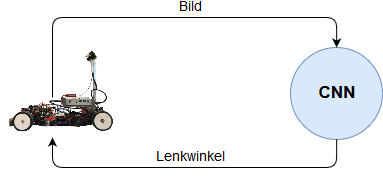
\includegraphics[scale=0.7]{figures/Aufbau.png}
	\caption{Eine tolle Grafik}
	\label{img:toll ist das}
\end{figure}


\section{Relevante Technik/Hintergrund}

\note{Hier werden kurz CNNs vorgestellt, Residual Technik erklärt}